\documentclass{article}

\usepackage[final]{neurips_2024}

\usepackage[utf8]{inputenc} % allow utf-8 input
\usepackage[T1]{fontenc}    % use 8-bit T1 fonts
\usepackage{hyperref}       % hyperlinks
\usepackage{url}            % simple URL typesetting
\usepackage{booktabs}       % professional-quality tables
\usepackage{amsfonts}       % blackboard math symbols
\usepackage{amsmath}        % math environments
\usepackage{nicefrac}       % compact symbols for 1/2, etc.
\usepackage{microtype}      % microtypography
\usepackage{xcolor}         % colors
\usepackage{natbib}
\usepackage{graphicx}
\usepackage{caption}
\captionsetup{font=small}

\bibliographystyle{plainnat}

\title{Final Report: Latent Reasoning in LLMs With Adaptive Halting Times}

\author{
  Faraz Mirza \\
  School of Computer Science\\
  Carnegie Mellon University\\
  \texttt{fmirza@andrew.cmu.edu} \\
  \And
  Brian Cho \\
  Language Technologies Institute \\
  Carnegie Mellon University \\
  \texttt{bcho2@andrew.cmu.edu} \\
}

\begin{document}
\maketitle

\begin{abstract}
Chain-of-thought prompting improves LLM reasoning but forces reasoning to occur through discrete tokens. \textsc{Coconut} \citep{coconut2025} addresses this by feeding hidden states directly back as input embeddings, enabling reasoning in continuous latent space. However, it allocates a fixed number of latent reasoning steps regardless of problem complexity. We propose augmenting \textsc{Coconut} with a learned adaptive halting head that dynamically determines how many latent steps to perform based on the hidden state at each step. On GSM8K, we show empirically that latent positions are redundant in proportion to problem complexity, and that a lightweight MLP halting head trained on task performance labels achieves 30.2\% accuracy while saving 26.8\% of latent steps --- outperforming an entropy-based heuristic baseline that saves only 13.1\% of latent steps at the same accuracy, and achieving 6.6 percentage points higher accuracy at matched compute budget.
\end{abstract}

\section{Introduction}

Chain-of-thought prompting has become a dominant approach for improving LLM reasoning, but forces models to reason entirely through discrete tokens. \textsc{Coconut} \citep{coconut2025} offers an alternative by feeding the transformer's final hidden state directly back as the next input embedding, allowing reasoning in continuous latent space. The hypothesis class of \textsc{Coconut} is a strict superset of CoT; empirically, it has been shown to outperform CoT on planning-intensive tasks while generating fewer tokens.

A key limitation is that \textsc{Coconut} allocates a fixed latent reasoning budget to every problem regardless of complexity. We propose replacing this with a learned adaptive halting head that produces a binary \textit{halt}/\textit{continue} decision at each latent step. Since the halting head can always learn to reproduce fixed-budget behavior, it is guaranteed to be at least as expressive as the original architecture.

We focus on GSM8K for two reasons. First, unlike ProsQA and PrOntoQA where latent tokens were explicitly designed during curriculum training to correspond to graph traversal hops, GSM8K's arithmetic reasoning steps do not decompose as cleanly into discrete sequential operations, making the fixed latent budget a less principled choice and adaptive halting more theoretically motivated. Second, GSM8K involves real-world scenarios described in natural language with numeric answers, and its reasoning steps span heterogeneous arithmetic operations rather than a single uniform operation as in graph traversal. This makes findings on GSM8K more likely to generalize beyond synthetic benchmarks.

During our literature search for pre-trained \textsc{Coconut} checkpoints, we also discovered an unpublished manuscript by \citet{martin2025curriculum} that directly challenges \textsc{Coconut}'s core claim on ProsQA: through careful ablation experiments, \citeauthor{martin2025curriculum} shows that a pause-token baseline trained under the same curriculum matches \textsc{Coconut}'s accuracy (96.6\% vs.\ 97.0\%, McNemar $p = 0.845$), suggesting the training curriculum rather than the continuous thought mechanism drives performance on that dataset. This further validated our focus on GSM8K, which \citet{martin2025curriculum} explicitly leaves open as a harder case where the mechanism may carry more weight.

Our contributions are threefold. First, we conduct a latent-state corruption analysis on GSM8K that empirically characterizes which latent positions are ``load-bearing'' --- that is, whose removal causes meaningful accuracy degradation --- and demonstrates that the number of critical positions scales with problem complexity (Section~\ref{sec:corruption}). Second, we establish an entropy-based early halting baseline that quantifies the accuracy--efficiency tradeoff and reveals the limitations of heuristic, non-adaptive halting (Section~\ref{sec:entropy}). Third, we train a learned halting head on task-performance labels and show it achieves substantially better efficiency at matched accuracy compared to the entropy heuristic (Section~\ref{sec:head}).

\section{Related Work}

There has been much recent work on LLM reasoning outside of language token space, as well as dynamic compute allocation to reasoning. Our work lies at the intersection of the two, and draws motivation from both to explore learned halting in latent or continuous thought.

\citet{pause2024} presented a simple approach to improving reasoning by delaying output and allowing more hidden-state processing. They appended learnable pause tokens to the input, delaying output extraction until the last pause is processed. Using a 1B-parameter model, they achieved performance improvements in several downstream tasks including reasoning and QA.

More directly related to our project, \citet{martin2025curriculum} conduct a factorial control study of \textsc{Coconut} on ProsQA, introducing curriculum-matched pause-token baselines to isolate the curriculum from the continuous thought mechanism. Their primary finding is that a single-pass pause baseline (M3) matches \textsc{Coconut}'s in-distribution accuracy at GPT-2 scale, while a multi-pass pause baseline (M4) reveals that sequential processing drives topological generalization and recycled content impairs chain-length extrapolation. Crucially, their work is restricted to ProsQA --- a synthetic, templated graph-traversal benchmark with fictional entities, binary answers, and a single uniform reasoning operation --- and explicitly leaves open whether their null result extends to harder, more naturalistic tasks such as GSM8K, where reasoning steps span heterogeneous arithmetic operations.

Notably, both \citet{pause2024} and \textsc{Coconut} have fixed compute allocations. Pause tokens are padded to a constant length, and \textsc{Coconut}'s latent budget is set in advance. More generally, the idea that neural models should learn how much computation to use has earlier roots in adaptive computation. \citet{act2016} introduced Adaptive Computation Time for recurrent networks, allowing the model to learn how many recurrent updates to apply to each input. \citet{universal2018} extended this idea to transformers by combining recurrent depth with adaptive halting, showing that computation depth itself can be input-dependent.

There has been strong empirical motivation for adaptive halting in recent literature on language-space reasoning. \citet{concise2025} identified two redundancy patterns in reasoning models, \textit{confidence deficit} and \textit{termination delay}, and introduced ConCISE, which reduces reasoning length by up to 50\% with minimal accuracy loss. Since ConCISE and related works operate in language space, our project extends this idea to latent space, where there are no explicit tokens to prune and halting decisions must be made from hidden state representations alone.

\section{Methods and Experiments}

This section describes each experiment in sequence, together with the findings that motivated the subsequent design choices. Our baseline is the original fixed-budget \textsc{Coconut} model \citep{coconut2025}; our main contribution is a learned halting adapter trained on top of a frozen checkpoint.

\paragraph{Checkpoint.} Due to the compute requirements of full \textsc{Coconut} training on GSM8K \citep{cobbe2021gsm8k, icot2024} (two sequential training phases, each taking many hours on multi-GPU hardware), we use a community checkpoint from HuggingFace (\texttt{jiviteshjn/coconut-checkpoints}, stage1\_resume/checkpoint\_13). This checkpoint corresponds to stage~3 of the GSM8K \textsc{Coconut} curriculum ($c_{\mathrm{thought}} = 2$, $k = 3$ steps replaced, 6 latent positions total) and achieves 36.4\% validation accuracy on GSM8K, consistent with the range reported across other public reproductions. We verified its behavior matches the \textsc{Coconut} paper's training dynamics before proceeding.

\subsection{Experiment A: Latent State Corruption Analysis}
\label{sec:corruption}

\paragraph{Motivation.} Before designing a halting mechanism, we ask: which latent positions are actually load-bearing? If computation is concentrated in a predictable subset of positions, an adaptive mechanism has clear targets for early stopping.

\paragraph{Method.} We follow the corruption methodology of \citet{martin2025curriculum}. For each of $N = 500$ validation samples, we re-run inference with selected latent positions replaced by calibrated Gaussian noise drawn to match the per-position mean and standard deviation of clean hidden states (estimated on 50 samples). We run three variants: (1) \textit{cumulative forward} corruption, replacing positions $0, \ldots, k$ for increasing $k$; (2) \textit{cumulative reverse} corruption, replacing positions $k, \ldots, 5$ for decreasing $k$; and (3) \textit{single-position} corruption, replacing only position $k$ for each $k \in \{0,\ldots,5\}$. We additionally run \textit{intra-step} experiments, corrupting only the first ($\{0, 2, 4\}$) or second ($\{1, 3, 5\}$) thought of each step, exploiting the $c_{\mathrm{thought}} = 2$ structure unique to GSM8K. All results are stratified by the number of gold reasoning steps.

\paragraph{Findings.} Three findings stand out. First, late positions are largely redundant: corrupting position~5 alone drops accuracy from 36.6\% to 32.6\%, while corrupting position~1 alone drops it to 8.8\% --- a 28pp difference for a single position. Second, position~1 (the second continuous thought of the first reasoning step) is catastrophically critical and difficulty-invariant: corrupting it drops easy (2-step) and medium (3--4 step) problems almost equally, while all other positions show difficulty-graded sensitivity. Third, the number of load-bearing positions scales directly with the number of gold reasoning steps. Problems requiring 2 gold steps maintain over 55\% accuracy under corruption of positions 3--5; problems requiring 4 gold steps show near-zero accuracy with those same positions corrupted. This establishes a clear empirical target for adaptive halting: the model should use approximately $\min(n_{\mathrm{steps}} \times c_{\mathrm{thought}},\, N_{\mathrm{latent}})$ passes per problem. See Figure~\ref{fig:corruption}.

These findings qualitatively distinguish GSM8K from \citeauthor{martin2025curriculum}'s ProsQA results, where computation was concentrated at a single middle position (position~3 of 6) consistent with a generic compute buffer. On GSM8K, the gradient of sensitivity from early to late positions and its dependence on problem complexity support the hypothesis that continuous thoughts carry reasoning-relevant content, providing a mechanistic basis for adaptive halting.

\begin{figure}[t]
    \centering
    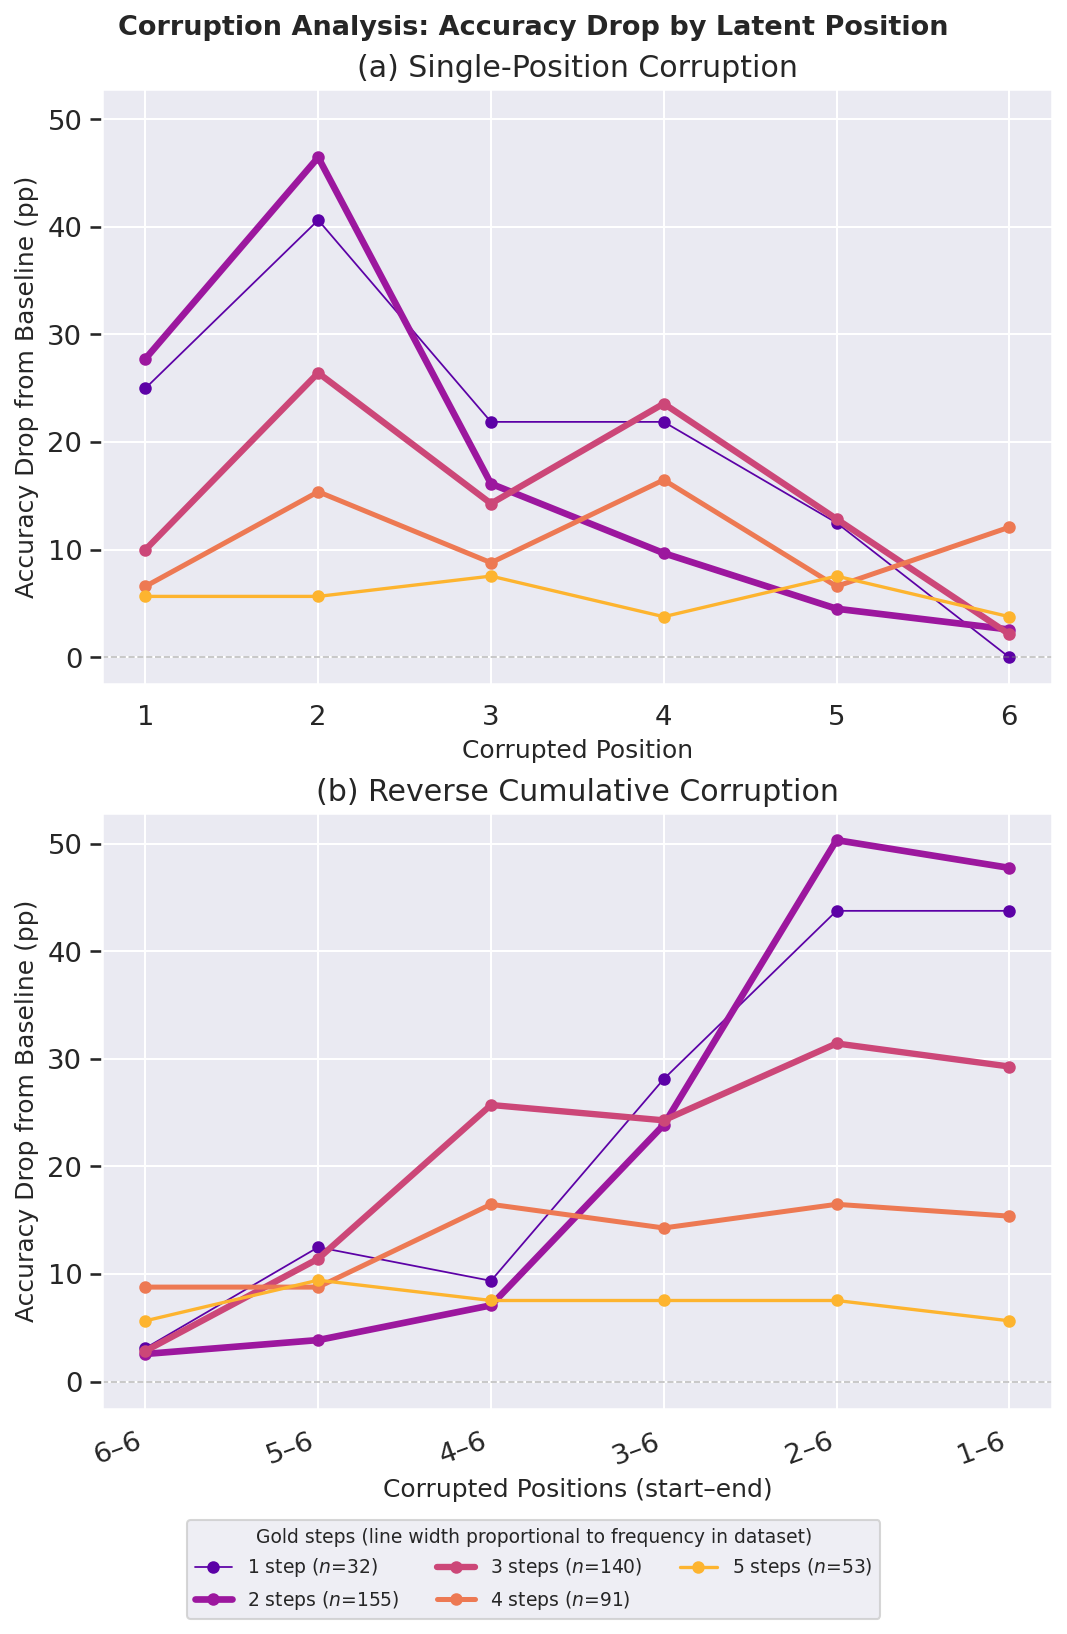
\includegraphics[width=\textwidth]{figures/corruption_superplot.png}
    \caption{\textbf{(a)} Accuracy drop from clean baseline when corrupting a single latent position, stratified by gold step count. Position~1 causes catastrophic, difficulty-invariant damage; late positions are nearly harmless for short problems. \textbf{(b, c)} Cumulative forward and reverse corruption curves by step count, showing the cliff position scales with gold step count.}
    \label{fig:corruption}
\end{figure}

\subsection{Experiment B: Entropy-Based Early Halting}
\label{sec:entropy}

\paragraph{Motivation.} Experiment A identifies which positions are redundant in hindsight. Experiment B asks: can we identify redundant positions at inference time using a simple signal, and what is the best accuracy--efficiency tradeoff achievable without training?

\paragraph{Method.} After each latent pass $k \geq 2$ (enforcing the critical first step), we compute the next-token entropy $H_k = -\sum_v p_v \log p_v$ over the full vocabulary from the current logits. If $H_k < \tau$ for threshold $\tau$, we halt and proceed to language generation using PAD mode: remaining latent positions retain their original \texttt{<|latent|>} token embeddings in the final pass. We sweep $\tau$ log-uniformly from 0.1 to 8.0 nats and record accuracy and average latent steps used for each threshold.

We also explored two alternative modes for handling skipped positions. \textit{Zero mode} replaced remaining positions with zero vectors, producing results 0.4--1.0pp below PAD mode, confirming that \texttt{<|latent|>} embeddings carry minimal information. \textit{EOT} (end-of-thought) \textit{mode} attempted to skip directly to the \texttt{<|end-latent|>} token using masked KV-cache attention, but produced substantially worse results ($\sim$5pp below PAD), indicating the model relies on attending over the full sequence structure it was trained with.

\paragraph{Findings.} The overall accuracy--latent-steps Pareto curve is a smooth linear decline with no plateau: every reduction in latent steps comes at a proportional accuracy cost. The entropy threshold cannot distinguish ``confidently correct'' from ``confidently wrong but in the wrong direction,'' making it fundamentally limited as a global signal.

Per-step-count analysis reveals a more nuanced picture. Problems with 1--2 gold steps can save approximately 20\% of latent steps for a single-digit accuracy drop; problems with 4+ gold steps show no favorable operating point. This asymmetry motivates a learned mechanism that conditions the halt decision on problem complexity.

\begin{figure}[t]
    \centering
    \includegraphics[width=\textwidth]{figures/halting_twopanel.png}
    \caption{\textbf{(a)} Overall accuracy vs.\ latent steps saved for the entropy threshold sweep. The orange star marks the learned halting head result. \textbf{(b)} Per-step count breakdown. Squares mark no-halt baselines at 0\% saved. Problems requiring fewer gold reasoning steps show a more favorable accuracy--efficiency tradeoff, with 1--2 step problems tolerating over 20\% latent step reduction with minimal accuracy loss.}
    \label{fig:pareto}
\end{figure}

\subsection{Experiment C: Learned Halting Head}
\label{sec:head}

\begin{figure}
    \centering
    \includegraphics[width=\linewidth]{figures/halt4.pdf}
    \caption{\textbf{Left:} Standard \textsc{Coconut} with fixed latent budget $k$. All latent positions receive recycled hidden states before answer generation. \textbf{Right:} Our adaptive variant. The HALT module (queried after each pass beyond a minimum of 2 steps) halts early when confident; remaining positions retain their original \texttt{<|latent|>} embeddings (shown in gray) and are processed in a single final pass before answer generation.}
    \label{fig:learned}
\end{figure}

\paragraph{Architecture.} The halting head is a single-hidden layer MLP with ReLU activation and sigmoid output:
\[
    p_{\mathrm{halt}} = \sigma\!\left(W_2\,\mathrm{ReLU}(W_1 h_k + b_1) + b_2\right),
\]
where $h_k \in \mathbb{R}^{768}$ is the last-layer hidden state at latent position $k$. The halting head receives the hidden state $h_k$ produced by the LLM at latent position $k$, before it is recycled as the input embedding for position $k+1$. The inner layer has dimension 128, giving approximately 99k parameters. The \textsc{Coconut} backbone (124M parameters) is frozen throughout.

\paragraph{Label generation.} For each of 12{,}000 stratified training samples, we run inference halting at each position $k \in \{2, 3, 4, 5\}$ and record whether the answer is correct. The optimal halt point $k^*$ is the smallest $k$ that gives a correct answer. Samples where no halt position gives a correct answer are discarded (24.5\% of samples); the remaining 9{,}054 samples provide labels. Hidden states are collected from a clean full forward pass.

\paragraph{Training.} Four training pairs $(h_k, \ell_k)$ for $k \in \{2, 3, 4, 5\}$ are constructed for each labeled sample (where $\ell_k = \mathbf{1}[k \geq k^*]$), giving 36{,}216 training pairs in total. The loss is weighted binary cross-entropy with class-frequency inverse weights, plus a normalized sparsity penalty:
\[
    \mathcal{L} = \mathbb{E}\!\left[w_{\ell}\,\mathrm{BCE}(p_{\mathrm{halt}}, \ell)\right] + \lambda \cdot \mathbb{E}\!\left[p_{\mathrm{halt}} \cdot \frac{k - 2}{3}\right],
\]
where $\lambda = 0.05$ encourages early halting. We train for 20 epochs with Adam ($\mathrm{lr} = 10^{-3}$, weight decay $10^{-4}$) and cosine annealing, selecting the checkpoint with best validation AUC. The minimum of 2 latent steps is enforced during inference.

\paragraph{Training dynamics.} Validation AUC converges to 0.908--0.909 from epoch~4 onward, with the best epoch at epoch~6 (AUC 0.909). Train loss continues declining beyond epoch~6 while val AUC remains flat, indicating the ceiling is the representational capacity of the frozen hidden states rather than insufficient data.

\section{Results}

Table~\ref{tab:main} summarizes our main results. We present two comparisons between the learned halting head and the entropy threshold baseline: one at matched latent steps saved and one at matched accuracy.

\begin{table}[h!]
\centering
\small
\begin{tabular}{lcccc}
\toprule
\textbf{Method} & \textbf{Accuracy} & \textbf{Avg latent steps} & \textbf{Latent steps saved} \\
\midrule
No halting (baseline) & 36.6\% & 6.00 & 0\% \\
\midrule
\multicolumn{4}{l}{(Matched latent steps saved)} \\
Entropy $\tau = 0.24$ & 23.6\% & 4.40 & 26.6\% \\
\textbf{Learned head} & \textbf{30.2\%} & \textbf{4.39} & \textbf{26.8\%} \\
\midrule
\multicolumn{4}{l}{(Matched accuracy)} \\
Entropy $\tau = 0.10$ & 30.2\% & 5.21 & 13.1\% \\
\textbf{Learned head} & \textbf{30.2\%} & \textbf{4.39} & \textbf{26.8\%} \\
\bottomrule
\end{tabular}
\caption{Main results on GSM8K validation (500 samples).
% At matched latent steps saved, the learned head achieves 6.6pp higher accuracy than the entropy threshold. At matched accuracy, it saves $2\times$ more latent steps.
The learned head achieves the same accuracy as the entropy threshold at $\tau{=}0.10$ while saving twice as many latent steps, and outperforms the entropy threshold with similar latent step reduction ($\tau{=}0.24$) by 6.6 points in accuracy.
}
\label{tab:main}
\end{table}

Table~\ref{tab:bysteps} breaks down the learned head's results by gold step count, revealing the adaptive allocation the head has learned.

\begin{table}[h!]
\centering
\small
\begin{tabular}{lcccc}
\toprule
\textbf{Gold steps} & \textbf{$n$} & \textbf{Accuracy (halt)} & \textbf{Accuracy (no halt)} & \textbf{Avg latent steps (halt)} \\
\midrule
1 & 32  & 37.5\% & 53.1\% & 3.41 \\
2 & 155 & 51.6\% & 60.6\% & 3.35 \\
3 & 140 & 27.1\% & 34.3\% & 4.48 \\
4 & 91  & 17.6\% & 20.9\% & 5.15 \\
5 & 53  &  9.4\% &  9.4\% & 5.70 \\
6+ & 29  &  0.0\% &  0.0\% & 5.90 \\
\bottomrule
\end{tabular}
\caption{Per-step-count breakdown for the learned halting head. Average latent steps used increases monotonically with gold step count, confirming the head allocates compute adaptively. Accuracy is well-preserved for 2--4 step problems relative to baseline.}
\label{tab:bysteps}
\end{table}

The adaptive allocation pattern is the key result: the head uses 3.35--3.41 latent steps on average for 1--2 step problems (saving 43--44\%), increasing to 5.15--5.70 for 4--5 step problems (saving 5--14\%). This monotonic scaling closely tracks the oracle pattern identified in Experiment A, where load-bearing positions scale with gold step count.

% \begin{figure}[t]
%     \centering
%     \includegraphics[width=0.55\textwidth]{figures/halting_adaptive_allocation.png}
%     \caption{Average latent steps used by the halting head at inference, stratified by gold reasoning step count. The head allocates compute proportionally to problem complexity, in contrast to entropy thresholds (shown for comparison) which apply a uniform decision criterion across all difficulty levels.}
%     \label{fig:adaptive}
% \end{figure}

\section{Discussion and Analysis}

\paragraph{Why does the halting head outperform the entropy threshold?}

The entropy threshold applies a single global criterion regardless of problem complexity. A low-entropy state after 2 latent passes may signal ``easy problem, done'' or ``hard problem, stuck at a confident but wrong answer'' --- and the threshold cannot distinguish these. The learned head, trained on task-performance labels, implicitly learns this distinction from the hidden state structure. The per-step-count breakdown (Table~\ref{tab:bysteps}) confirms the difference: the entropy threshold at $\tau = 0.24$ assigns an average of 4.4 latent steps uniformly across difficulties, while the head assigns 3.35--5.90 in a monotone pattern that matches problem complexity.

\paragraph{The representation ceiling.}

Val AUC converged to 0.908 from epoch~4 regardless of further training, indicating the limit is the information content of the frozen hidden states rather than the classifier's capacity. The hidden states at each latent pass were produced by a model trained with a fixed-budget language modeling objective, without any signal encouraging them to be informative for halting decisions. This manifests most clearly in the 1-step problem failure mode: the head allocates 3.41 latent steps on average to 1-step problems (vs.\ the oracle of 2), slightly underperforming the entropy threshold on this subgroup. This suggests the hidden states after 2 passes do not reliably encode ``this problem needed only one reasoning step.''

\paragraph{Relation to \citet{martin2025curriculum}.}

\citeauthor{martin2025curriculum} show that on ProsQA at GPT-2 scale, continuous thought representations are largely interchangeable with fixed pause embeddings --- the curriculum, not the mechanism, drives accuracy. Our corruption analysis on GSM8K reveals a qualitatively different pattern: latent positions show difficulty-graded sensitivity rather than a concentrated cliff at a single position, and the gradient of criticality correlates with gold step count. This suggests that on GSM8K, the continuous thought representations carry more reasoning-relevant structure than on ProsQA, providing a mechanistic basis for why our adaptive head can learn a meaningful halting signal from those representations. These findings are complementary: \citeauthor{martin2025curriculum} characterize when the mechanism does not matter; our work provides evidence for when and how it can be exploited.

\paragraph{Limitations.}

Our evaluation uses a single community checkpoint trained with a single seed, which limits the statistical reliability of our results. The checkpoint is at stage~3 of the GSM8K curriculum, not the final stage; a fully trained checkpoint might show different redundancy patterns. The halting head was trained only on solvable problems (75.5\% of samples), which may bias it toward the difficulty distribution of solvable cases. Finally, all experiments are at GPT-2 124M scale, and our conclusions may not generalize to larger models.

\paragraph{Future work.}

Three directions are most promising. First, an \textit{attention-based halting module} that attends over the trajectory of hidden states $\{h_0, \ldots, h_k\}$ rather than a single snapshot could overcome the representation ceiling by observing how much the hidden state is changing across passes --- a natural signal for ``am I still making progress?'' Second, \textit{joint backbone fine-tuning} with the halting objective would allow the \textsc{Coconut} representations to develop halting-informative structure, potentially breaking through the 0.91 AUC ceiling. Third, the \textit{scaling hypothesis} is the most compelling long-term direction: at larger model scale, hidden states carry richer representations, each latent pass does more meaningful computation, and the range of solvable problems expands. \citet{martin2025curriculum} explicitly note their null result is specific to GPT-2 124M scale; our adaptive halting results establish an infrastructure for testing whether the mechanism --- and the efficiency gains from adapting its budget --- become more significant at LLaMA or GPT-4 class scale.

\bibliography{references}

\end{document}